\chapter{Implementation}

\section{Level Set Algorithm}\label{levelsetalgorithm}

\subsection{Upwinding}
Equation \eqref{eq:levelsetequation}, the level set equation, needs to be discretized for both sequential and parallel computation. This is done using the \textit{up-wind} differencing scheme. The following explanation of \textit{upwinding} is from \cite{osher2003lsm}.

A first order accurate method for time discretization of equation \eqref{eq:levelsetequation}, is given by the forward Euler method, from \cite{osher2003lsm}:

\begin{equation}
\frac{\phi^{t+\Delta t}-\phi^t}{\Delta t} +F^{t}\cdot{\nabla{\phi^{t}}} = 0
\label{eq:euler1}
\end{equation}

where $\phi^{t}$ represents the current values of $\phi$ at time $t$, $F^{t}$ represents the velocity field at time $t$, and  $\nabla{\phi^{t}}$ represents the values of the gradient of $\phi$ at time $t$. When computing the gradient, a great deal of care must be taken with regards to the spatial derivatives of $\phi$. This is best exemplified by considering the expanded form of equation \eqref{eq:euler1}.

\begin{equation}
\frac{\phi^{t+\Delta t}-\phi^t}{\Delta t} +u^{t}\phi_x^t+v^{t}\phi_y^t+w^{t}\phi_z^t = 0
\label{eq:euler2}
\end{equation}

For simplicity, consider the one dimensional form of equation \eqref{eq:euler2} at a specific grid point $x_i$ 

\begin{equation}
\frac{\phi^{t+\Delta t}-\phi^t}{\Delta t} +u_i^{t}(\phi_x)_i^t = 0
\label{eq:euler3}
\end{equation}

where $(\phi_x)_i$ is the spatial derivative of $\phi$ at $x_i$. The method of characteristics indicates whether to use a forward difference or backwards difference for $\phi$ based on the sign of $u_i$ at the point $x_i$. If $u_i > 0$, the values of $\phi$ are moving from left to right, and therefore backwards difference methods ($D_x^-$) should be used. Conversely, if $u_i<0$, forward difference methods ($D_x^+$) should be used to approximate $\phi_x$. It is this process of choosing which approximation for the spatial derivative of $\phi$ to use based on the sign of $u_i$ that is known as \textit{upwinding}. 

Extending this to three dimensions, from \cite{Lefohn04astreaming}, results in the derivatives below required for the level set equation update. 

\begin{eqnarray}
	D_x &=& (u_{i+1,j,k}-u_{i-1,j,k})/2 \nonumber\\
	D_y &=& (u_{i,j+1,k}-u_{i,j-1,k})/2 \nonumber\\
	D_z &=& (u_{i,j,k+1}-u_{i,j,k-1})/2 \nonumber\\
	D_x^+ &=& u_{i+1,j,k}-u_{i,j,k} \nonumber\\
	D_y^+ &=& u_{i,j+1,k}-u_{i,j,k} \nonumber\\
	D_z^+ &=& u_{i,j,k+1}-u_{i,j,k} \nonumber\\
	D_x^- &=& u_{i,j,k}-u_{i-1,j,k} \nonumber\\
	D_y^- &=& u_{i,j,k}-u_{i,j-1,k} \nonumber\\
	D_z^- &=& u_{i,j,k}-u_{i,j,k-1} \nonumber\\
\end{eqnarray}

$\nabla\phi$ is approximated using the upwind scheme.

\begin{eqnarray}
\nabla\phi_{\max} &=& \left[
  \begin{array}{ c }
     \sqrt{\max(D_x^+, 0)^2 + \max(-D_x^+,0)^2}  \\[2em]
     \sqrt{\max(D_y^+, 0)^2 + \max(-D_y^+,0)^2}  \\[2em]
     \sqrt{\max(D_z^+, 0)^2 + \max(-D_z^+,0)^2}  
  \end{array} \right] \\[2em]
\nabla\phi_{\min} &=& \left[
  \begin{array}{ c }
     \sqrt{\min(D_x^+, 0)^2 + \min(-D_x^+,0)^2}  \\[2em]
     \sqrt{\min(D_y^+, 0)^2 + \min(-D_y^+,0)^2}  \\[2em]
     \sqrt{\min(D_z^+, 0)^2 + \min(-D_z^+,0)^2} 
  \end{array} \right] 
\end{eqnarray}

Finally, depending on whether $F_{i,j,k} > 0$ or $F_{i,j,k} < 0$, $\nabla\phi$ is 

\begin{equation}
\nabla\phi = \left\{ 
\begin{array}{l l}
  ||\nabla\phi_{\max}||_2 & \quad \mbox{if $F_{i,j,k} > 0$}\\
  ||\nabla\phi_{\min}||_2 & \quad \mbox{if $F_{i,j,k} < 0$}\\ \end{array} \right.
\label{eq:finalchoice}
\end{equation}

\begin{equation}
\phi(t+\Delta t) =\phi(t) + \Delta t F|\nabla\phi|
\label{eq:phi}
\end{equation}

The speed term $F$, as discussed before, is based on the pixel intensity values and curvature values. 

\subsection{Curvature}
Curvature is computed based on the values of the current level set using the derivatives below. In two dimensions only the first two derivatives are required, alongside the derivatives defined previously. In three dimensions, all the derivatives below are required.

\begin{eqnarray}
	D_x^{+y} &=& (u_{i+1,j+1,k}-u_{i-1,j+1,k})/2 \nonumber\\
	D_x^{-y} &=& (u_{i+1,j-1,k}-u_{i-1,j-1,k})/2 \nonumber\\
	D_x^{+z} &=& (u_{i+1,j,k+1}-u_{i-1,j,k+1})/2 \nonumber\\
	D_x^{-z} &=& (u_{i+1,j,k-1}-u_{i-1,j,k-1})/2 \nonumber\\
	D_y^{+x} &=& (u_{i+1,j+1,k}-u_{i+1,j-1,k})/2 \nonumber\\
	D_y^{-x} &=& (u_{i-1,j+1,k}-u_{i-1,j-1,k})/2 \nonumber\\
	D_y^{+z} &=& (u_{i,j+1,k+1}-u_{i,j-1,k+1})/2 \nonumber\\
	D_y^{-z} &=& (u_{i,j+1,k-1}-u_{i,j-1,k-1})/2 \nonumber\\
	D_z^{+x} &=& (u_{i+1,j,k+1}-u_{i+1,j,k-1})/2 \nonumber\\
	D_z^{-x} &=& (u_{i-1,j,k+1}-u_{i-1,j,k-1})/2 \nonumber\\
	D_z^{+y} &=& (u_{i,j+1,k+1}-u_{i,j+1,k-1})/2 \nonumber\\
	D_z^{-y} &=& (u_{i,j-1,k+1}-u_{i,j-1,k-1})/2 \nonumber\\
\end{eqnarray}

Using the \textit{difference of normals} method from \cite{Lefohn04astreaming}, curvature is computed using the above derivates with the two normals $\textbf{n}^+$ and $\textbf{n}^-$.

\begin{eqnarray}
\textbf{n}^+ &=& \left[
  \begin{array}{ c }
     \frac{D_x^+}{\sqrt{(D_x^+)^2 + {\left(\frac{D_y^{+x}+D_y}{2}\right)}^2 +{\left(\frac{D_z^{+x}+D_z}{2}\right)}^2  }}  \\[2em]
     \frac{D_y^+}{\sqrt{(D_y^+)^2 + {\left(\frac{D_x^{+y}+D_x}{2}\right)}^2 +{\left(\frac{D_z^{+y}+D_z}{2}\right)}^2  }}  \\[2em]
     \frac{D_z^+}{\sqrt{(D_z^+)^2 + {\left(\frac{D_y^{+z}+D_x}{2}\right)}^2 +{\left(\frac{D_y^{+z}+D_y}{2}\right)}^2  }}  
  \end{array} \right] \\[2em]
\textbf{n}^- &=& \left[
  \begin{array}{ c }
     \frac{D_x^-}{\sqrt{(D_x^-)^2 + {\left(\frac{D_y^{-x}+D_y}{2}\right)}^2 +{\left(\frac{D_z^{-x}+D_z}{2}\right)}^2  }}  \\[2em]
     \frac{D_y^-}{\sqrt{(D_y^-)^2 + {\left(\frac{D_x^{-y}+D_x}{2}\right)}^2 +{\left(\frac{D_z^{-y}+D_z}{2}\right)}^2  }}  \\[2em]
     \frac{D_z^-}{\sqrt{(D_z^-)^2 + {\left(\frac{D_y^{-z}+D_x}{2}\right)}^2 +{\left(\frac{D_y^{-z}+D_y}{2}\right)}^2  }}  
  \end{array} \right] 
\label{eq:n}
\end{eqnarray}

The two normals are used to compute divergence, allowing for mean curvature to be computed as shown below in equation \eqref{eq:curv}.

\begin{equation}
H = \frac{1}{2}\nabla\cdot\frac{\nabla\phi}{|\nabla\phi|} = \frac{1}{2}((\textbf{n}_x^+ - \textbf{n}_x^-)+(\textbf{n}_y^+ - \textbf{n}_y^-)+(\textbf{n}_z^+ - \textbf{n}_z^-))
\label{eq:curv}
\end{equation}

\subsection{Stability}
From \cite{osher2003lsm}, a finite difference approximation to a linear partial differential equation is convergent if and only if it is both consistent and stable. Stability implies that small errors in the solution are not amplified during iteration. Stability is enforced using the Courant-Friedreichs-Lewy (CFL) condition which states the numerical wave speed must be greater than the physical wave speed, i.e. $\Delta x/\Delta t>|u|$. Rearranging, we have

\begin{equation}
\Delta t < \frac{\Delta x}{max\left\{|u|\right\}}
\label{eq:cfl}
\end{equation}

which is usually implemented, through variants of equation \eqref{eq:cfl}, by choosing a \textit{CFL number} that lies between 0 and 1 to further guarentee stability.

Another measure taken to ensure stability is the inclusion of a floating point relative accuracy term in the denominator of any fractions to avoid singularity errors as the denominator tends to zero. This is done in equations \eqref{eq:n} to ensure that $\textbf{n}$ does not tend to infinity if the square root is zero.

\section{2D Sequential Implementation}
Two dimensional implementations of the code in MATLAB, C and then CUDA were the first to be written. Once these had been optimized, three dimensional implementations were coded. The following pseudocode outlines the structure of the MATLAB, C and CUDA implementations, with only minor differences between the different versions.

\begin{algorithm}[h]
\dontprintsemicolon
\KwIn{Feature Image $I$, Initial Mask $m$, Threshold $T$, Range $\epsilon$, Iterations $N$}
\KwOut{Segmentation Result}
\BlankLine
\SetLine
Initialise $\phi_0$\ to S.D.F from mask $m$\;
Calculate Data Speed Term $D(I)= \epsilon - |I-T|$\;
\ForAll{$N$ Iterations}{
Calculate First Order Derivatives $D_x^{(\pm)},D_y^{(\pm)},D_z^{(\pm)}$ \;
Calculate Second Order Derivatives $D_x^{(\pm y,z)},D_y^{(\pm x,z)}...D_z^{(\pm x,y)}$ \;
Calculate Curvature Terms $\textbf{n}^+ , \textbf{n}^-$\;
Calculate Gradient $\nabla{\phi}$\;
Calculate Speed Term $F=\alpha D(\bar{x})  + (1-\alpha)\nabla \cdot{\frac{\nabla{\phi}}{|\nabla{\phi|}}}$\;
Update Level Set Function $\phi(t+\Delta t) =\phi(t) + \Delta t F|\nabla\phi|$\;
\If{Iterations \% 50 == 0}{
Reinitialise $\phi$ to S.D.F
}
}
\caption{Pseudocode for Level Set Segmentation}\label{alg:alg}
\end{algorithm}


	\subsection{Matlab}
The first task was to write code in MATLAB to segment two dimensional greyscale images. The MATLAB Image Processing Toolbox provides many functions (such as the ability to load, resample and filter images, compute distance transforms and easily visualise the level set evolution) which kept the code reasonably concise. 

The code is split into two files (a launcher and a kernel), in order to seperate the initialisation and level set update code. The launcher handles the image loading and resampling, with the functions \texttt{imread} and \texttt{imresize}. The user specifies parameters for threshold values $T$, range $\epsilon$ and curvature weighting $\alpha$, runs the launcher and then proceeds to draw a closed polygon that will form the initial mask (providing some basic interactivity). 

\begin{figure}[h]
	\centering
		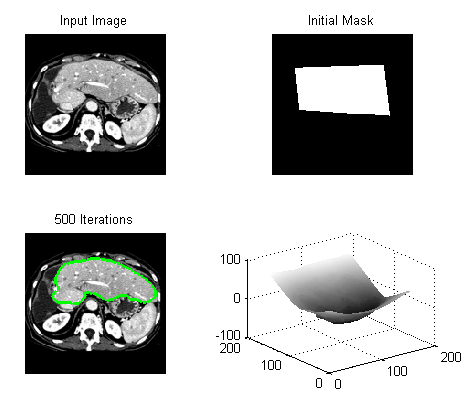
\includegraphics[scale=0.6]{images/matlab.png}
	\caption{MATLAB user interface showing four subfigures with the input image, the initial mask, the current zero level set interface superimposed on the input image and the current level set surface in 3D}
	\label{fig:matlab}
\end{figure}

The level set function $\phi$ is then initialised to a signed distance function of this mask, and iteration of the level set equation begins for a fixed number of iterations (also user-definable). Reinitialisation of the level set is performed once every 50 iterations, and the current level set contour and surface are displayed every 20 iterations.

The derivatives are calculated by subtracting shifted matrices of $\phi$ from $\phi$ (or vice-versa). Note how derivatives are not calculated in an element by element fashion.

Finally, the user has the option of downsampling the input image in order to speed up the computation.

CFL

	\subsection{C}
Initially C code was written to most closely mirror the MATLAB code. The feature image, level set function, and derivatives were stored in memory as one dimensional arrays. These arrays were stepped through by nested for loops, looping $i$ looping $j$. To go from the two dimensional $i,j$ indices to a one dimensional index \textit{ind}, the equation $\textrm{ind} = j \times \textrm{imageW} +i$ These for loops computed the derivatives serially, as shown in the pseudocode for algorithm \ref{alg:forloop}. This approach favoured itself well to being optimized at a low level using pointers to quickly step through the data. It was inefficient from a memory management perspective, with the derivative arrays taking up large amounts of memory for large image sizes, and also continuosly being allocated and freed at each iteration.

\begin{algorithm}[h]
\dontprintsemicolon
\ForAll{$i,j$}{
Calculate $D_x$\;
}
\ForAll{$i,j$}{
Calculate $D_y$\;
}
\ForAll{$i,j$}{
Calculate $D_z$\;
}
\ForAll{$i,j$}{
Calculate $D_x^+$\;
}
\BlankLine
...\;
\BlankLine
Update Level Set Function $\phi(t+\Delta t) =\phi(t) + \Delta t F|\nabla\phi|$\;
\caption{Pseudocode for Version 1 of Sequential C Code}\label{alg:forloop}
\end{algorithm}

This C implementation did not feature the versatility of the MATLAB implementation as it only accepted bitmap images as the input for the feature image. The loader function for the bitmap images (\texttt{bmploader.cpp}) is from the NVIDIA CUDA SDK image processing examples. It also did not feature any image resizing functions, as the focus was on optimization of the code and not versatility of inputs.

Wheras the MATLAB code used shifts of the matrix $\phi$ to calculate derivatives, in C the level set function $\phi$ was being stepped through in an element by element fashion. Therefore many boundary conditions had to be placed in order to ensure that derivatives took the value zero at certain boundaries. For example the forward difference derivative $D_x^+ =u_{i+1,j}-u_{i,j}$ must equal zero when $i=\textrm{imageW}$ as there is no $u_{i+1,j}$ term. The complexity of this task increases in three dimensions as there are six boundaries instead of four boundaries to condition for.

Restructuring the code for parallel computation of derivatives (using only one for loop) laid the framework for parallelization in CUDA, and only had a minor impact on performance. In this case all the derivatives are calculated at the same time at a given pixel, as shown below in algorithm \ref{alg:forloop2}. Also, the derivatives no longer needed to be stored in memory as arrays, and were simply floating point variables declared at each iteration. These two changes condensed the C code greatly.


\begin{algorithm}[h]
\dontprintsemicolon
\ForAll{$i,j$}{
Calculate $D_x$\;
Calculate $D_y$\;
Calculate $D_z$\;
Calculate $D_x^+$\;
\BlankLine
...\;
}
\BlankLine
Update Level Set Function $\phi(t+\Delta t) =\phi(t) + \Delta t F|\nabla\phi|$\;
\caption{Pseudocode for Version 2 of Sequential C Code}\label{alg:forloop2}
\end{algorithm}

For the distance transform initialization and reinitialization proceedures a seperate function was called. This is the "sedt2d" (Signed Euclidean Distance Transform in 2D) function written by Timothy Terriberry.

GLUT, LACK OF CFL

\section{2D Parallel Implemention}
	\subsection{Unoptimized Version}
The first parallel implementation followed the structure shown in the pseudocode below. In CUDA, it is assumed that both the host and device maintain their own DRAM \cite{cuda}. Host memory is allocated as before using \texttt{malloc} and device memory is allocated using \texttt{cudaMalloc}. As memory transfers either from host to device or device to host are particularly slow, it is recommended to keep the number of transfers to a minimum. Therefore most CUDA programs follow a similar strucutre of initialization, memory transfer, compute, memory transfer. 

Unfortunately the algorithm for computing signed distance transforms is not executed in CUDA (and creating one from scratch would have been beyond the scope of this project), therefore required device to host memory transfer every time reinitialization was required. Of course, when timing it is possible to stop and start timers during this process.

	
\begin{algorithm}[h]
\dontprintsemicolon
\BlankLine
\SetLine
Initialise $\phi_0, D$ on host memory\;
Allocate memory for $\phi_n ,\phi_{n+1}, D$ on device\;
Copy $\phi_0 , D$ from host to device\;
\ForAll{$N$ Iterations}{
Execute Level Set Update CUDA Kernel $\phi_{n+1} =\phi_n + \Delta t F|\nabla\phi_n|$\;
Swap pointers of $\phi_n ,\phi_{n+1}$\;
\If{Iterations \% 50 == 0}{
Copy $\phi$ from device to host\;
Reinitialise $\phi$ to S.D.F\;
Copy $\phi$ from host to device\;
}
}
Copy $\phi$ from device to host\;
\caption{Parallel Implementation Pseudocode}\label{alg:cuda1}
\end{algorithm}	

CUDA threads are assigned a unique thread ID that identifies its location within the threadblock and grid. This provides a natural way to invoke computation across the image and level set domain, by using the thread IDs for addressing.  This is best explained using the table below. Assume our image has dimensions $4\times 4$ and the block size is $2 \times 2$. Invoking the kernel with a grid size of $2 \times 2$ results in the 16 threads shown in table \ref{table:threads}, in the form (\texttt{threadIdx.y},\texttt{threadIdx.x}). These threads are grouped into blocks of four, as shown in table \ref{table:blocks}, in the form (\texttt{blockIdx.y},\texttt{blockIdx.x}). 
\begin{center}
  \begin{tabular}{ | c | c || c | c |}
    \hline
    (0,0) & (0,1) & (0,1) & (0,1) \\ \hline
    (1,0) & (1,1) & (1,0) & (1,1) \\ \hline\hline
    (0,0) & (0,1) & (0,0) & (0,1) \\ \hline
    (1,0) & (1,1) & (1,0) & (1,1) \\
    \label{table:threads}
  \end{tabular}
\end{center}

\begin{center}
  \begin{tabular}{ | c | c |}
    \hline
    (0,0) & (0,1)  \\ \hline
    (1,0) & (1,1)  \\ 
    \label{table:blocks}
  \end{tabular}
\end{center}

As each thread has access to its own \texttt{threadIdx} and \texttt{blockIdx} global indices ($i,j$) can be determined using the equations

\begin{center}
\begin{verbatim}
	int c= blockIdx.x * blockDim.x + threadIdx.x;
	int r= blockIdx.y * blockDim.y + threadIdx.y;
\end{verbatim}
\end{center}

where \texttt{blockDim.x} and \texttt{blockDim.y} represent the dimensions of the block (which in this case are both equal to 2).

	\subsection{Shared Memory}
	
	
